%%%%%%%%%%%%%%%%%%%% file paper.tex %%%%%%%%%%%%%%%%%%%%%
% ICSC 2026 submission, based on icsc2026_template.tex (llncs.cls)
%%%%%%%%%%%%%%%%%%%%%%%%%%%%%%%%%%%%%%%%%%%%%%%%%%%%%%%%%

\documentclass[runningheads,a4paper]{llncs}

\usepackage{amssymb}
\setcounter{tocdepth}{3}
\usepackage{graphicx}
\usepackage{tikz}
\usetikzlibrary{arrows.meta,calc,fit,positioning}
\usepackage{hyperref}
\usepackage[margin=1.1in]{geometry}
\hypersetup{hidelinks}
\newcommand{\keywords}[1]{\par\addvspace\baselineskip
\noindent\keywordname\enspace\ignorespaces#1}

% Supplementary material (full example artifacts) archived on Zenodo.
% Replace the placeholder DOI with the real one before submission.
\newcommand{\supplementaryurl}{https://doi.org/10.5281/zenodo.XXXXXXX}

\pagestyle{headings}

\begin{document}

\mainmatter

\title{One Timeline, Many Renderings:\\ A Wolfram Language Paclet\\ for Heterogeneous Musical Output}

\titlerunning{One Timeline, Many Renderings}

% TO GUARANTEE THE DOUBLE BLIND REVIEW PROCESS, GENERIC
% AUTHOR NAMES AND INSTITUTION ARE KEPT
\author{AuthorA \and AuthorB \and AuthorC}
\authorrunning{AuthorA et al.}
\institute{InstituteA}

\maketitle

\begin{abstract}
Algorithmic composition rarely ends in a single medium: the same musical plan
may need to become a Csound score for synthesis, engraved notation for
performers, a real-time control stream, and a click track for rehearsal.
Authored or repaired separately, these timelines drift apart. We present
Temporal System, a Wolfram Language paclet that treats heterogeneous output as
a projection problem: one immutable store of typed musical entities, placed on
a rational beat timeline, is compiled by per-backend renderers into Csound
(electroacoustic and synthesis), MusicXML (symbolic score, in beta against
MusicXML~4.0), and OSC (a pre-rendered control stream for real-time dispatch)
artifacts that stay synchronous because they share one store. We describe the design decisions, the
anatomy (temporal, semantic, and rendering layers; fourteen modules), and the
renderers. Particular attention goes to Csound,
which fixes the rendering idiom: compiled tempo maps yield onset and duration
seconds only at render time, session tuning yields p4 frequencies, curve
entities compile to k-rate control signals bound to score p-fields, and
orchestras remain ordinary \texttt{.orc} files addressed by stable named
instruments---the score--orchestra separation Csound inherits from the
\textsc{music~n} family. A click-track backend derives rehearsal audio from the
same meter and tempo and reuses the Csound serializer---how cheaply a further
projection follows once the temporal core is shared.
\keywords{Csound, algorithmic composition, music representation, Wolfram
Language, click track}
\end{abstract}


\section{Introduction}

Long before rendering became plural, computing composers had already separated
structure from sound. At Bell Labs, Tenney generated note lists for the
\textsc{music~n} programs \cite{tenney,mathews}; in Utrecht, Koenig's
\emph{Project~1} and \emph{Project~2} computed a piece as tables realized at a
later stage---players, the studio, and in his last works Csound itself
\cite{koenig}. In both, the program owns \emph{time and structure} and a
separate system owns \emph{sound}: the orchestra--score split Csound
institutionalizes \cite{csoundbook}.

Contemporary practice multiplies the realization stages: a mixed work may need
a \texttt{.csd} for synthesis, MusicXML for engraving, a timed control stream
for live electronics, and a click track for performers. These encode time
differently---seconds, divisions per quarter, milliseconds, samples---so
maintaining them by hand means maintaining four diverging timelines.
Computer-assisted composition environments have long addressed parts of this
\cite{openmusic,taube}; Temporal System~\cite{wolfram} makes one authored
timeline the only source of truth and demotes every output file to a derived
artifact.

One model feeding many outputs is well established. \emph{music21} exports a
single object model to MusicXML, MIDI, Lilypond and text \cite{music21};
\emph{abjad} drives Lilypond from a persistent Python score model
\cite{abjad}; MEI encodes a canonical score that Verovio projects to many
targets \cite{mei,verovio}; \emph{bach} and \emph{cage} carry a
score/timeline abstraction into Max for real-time realization \cite{bach}.
These are organized around notation or a single real-time host. Exact
rational time is not new on its own either: \emph{TidalCycles} represents
patterns as functions over cycles of exact rational time \cite{tidal}, but in
the service of live-coded pattern scheduling dispatched to a synthesis host,
not of offline serialization to heterogeneous files. Temporal System's
contribution is the \emph{combination}: one beat-space substrate of exact
Rationals (musical, not clock, time) that simultaneously feeds several
restrictive, heterogeneous serializers, with conversion to seconds, hertz and
samples deferred to each renderer. The host language makes
this practical: store, tempo-map inversion, session tuning and per-backend
contracts are all Wolfram Language, in which rationals stay exact,
transformations compose, and a vast built-in library (including the paclet's own
timeline graphics) sits where the timeline is authored---so authoring the piece
and compiling its every projection share one language, not a chain of programs.

Temporal System's design decisions are few and strict: (i)~events live in an immutable
store of typed entities whose onsets are exact Rationals in beat space,
never seconds; (ii)~meter is authored state, never inferred from durations;
(iii)~reference tuning is a session parameter, never a constant in
conversion code; (iv)~the paclet generates \emph{scores only}---synthesis
instruments remain external \texttt{.orc} files, as in Koenig's and Tenney's
workflows; (v)~the shared store is permissive, while each renderer enforces
a restrictive contract for its own payload.

One trade-off is worth stating. Authoring requires Wolfram Language, a
commercial environment (a free Wolfram Engine covers development and
non-commercial use), whereas Csound and much of its ecosystem are open-source.
The dependency is confined to authoring: the emitted artifacts---the
\texttt{.csd} with its \texttt{\#include}d \texttt{.orc} files, MusicXML, and
the OSC JSON---are plain text in open formats needing no Wolfram runtime to
compile, engrave, or dispatch.

\section{Anatomy of the Paclet}

The paclet comprises fourteen modules exposing 80 public functions in three
layers: \texttt{core} (entities, store, tempo, session), \texttt{rendering}
(dispatcher and four backends), and \texttt{util} (pitch, rhythm, dynamics,
validation, timeline graphics). Layers~I (temporal) and~II (semantic) are
backend-agnostic; Layer~III holds one restrictive contract per backend, and
adding a backend adds a contract there without ever touching Layers~I--II. All
functions are pure; store operations return new stores.

\textbf{Layer I.} Tempo is authored as a \emph{tempoSpec}, an ordered list
of $\{$beat, BPM$\}$ points, and compiled to a piecewise-linear
\emph{tempoMap} in $\{$beat, seconds$\}$ form with exact analytical
inversion. Onsets and durations are Rationals in musical duration space;
conversion to seconds or samples happens only inside renderers.

\textbf{Layer II.} The store groups entities by type
(\texttt{stemData[type][id]}, $O(1)$ typed access; rendering is linear in the
event count, so the model scales to large scores) across seven implemented
entity types (note, rest, trigger, curve, state, marker, annotation), with four
more (process, interval, trajectory, gesture) declared for future use. A note carries pitch (spelling plus cents, MIDI float,
or frequency), duration, dynamic, and a \texttt{rendering} association keyed by
backend id---the one place backend-specific payloads travel with the entity.
Meter is a state entity: measure structure is authored, not guessed. A session
configuration carries everything a renderer may not hardcode, starting with
\texttt{tuningA4} (default 440~Hz, freely reassignable).

\textbf{Layer III.} Constructors validate only the shared shape and require each
\texttt{rendering[backend]} payload to be an association whose keys belong to the
backend contract; malformed Csound payloads are therefore Csound contract
errors, local to one renderer, and each backend declares a fallback policy
(warn, approximate) for material it cannot express.

The paclet also inspects itself: \texttt{drawTimeline} renders any stemData as
lane-based graphics with the metric grid derived from the authored meter
entities (Fig.~\ref{fig:timeline}), from a single function call with no external
tool. Every fixture in the Csound suite renders to a \texttt{.csd} that Csound
compiles without error, and its rendered audio was auditioned.

\begin{figure}
\centering
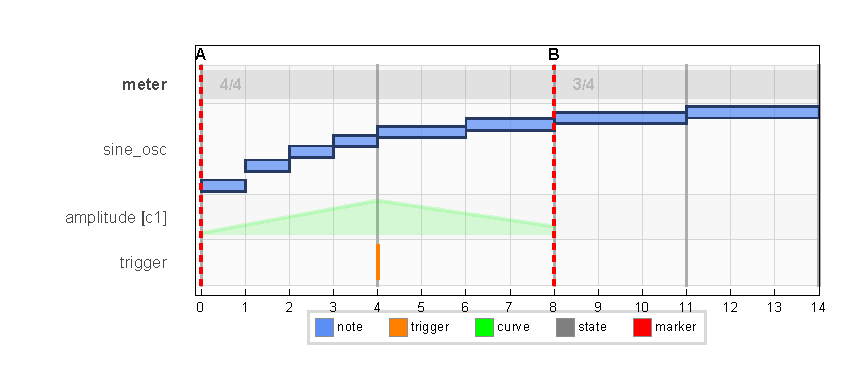
\includegraphics[width=0.66\linewidth]{figures/timeline_export}
\caption{A timeline exported directly by the paclet
(\texttt{drawTimeline}): the Csound suite's most complex
fixture---sixteen \texttt{sine\_osc} notes (several with cent offsets),
eight \texttt{click} hits, four triggers, six overlapping amplitude/pan
curves, section markers, and a $4/4 \to 5/8 \to 7/8 \to 3/4$ meter grid. A
stress fixture exercising many entity types at once, not a representative
composition.}
\label{fig:timeline}
\end{figure}

\section{The Implemented Renderers}

A backend is data: an association with an id, a renderer, a serializer, the
primitive types it emits, and a fallback policy. The generic dispatcher
\texttt{renderTo[stemData, tempo, backend, config, registry]} is the single
entry point. Four backends exist. \emph{Csound} compiles the whole stemData to
score and orchestra primitives (Sect.~\ref{sec:csound}); \emph{Click} derives a
standalone rehearsal track from meter and tempo alone (Sect.~\ref{sec:click}).
\emph{MusicXML} builds measures from meter state, splits notes at barlines into
tied fragments, and validates measure capacity, part coverage, and tie and
chord integrity; it is an explicitly lossy projection with a declared coverage
profile \cite{good}, currently in beta, emitting MusicXML~4.0 (partwise) and
checked by round-tripping through Dorico for tie, meter and part-separation
fidelity. \emph{OSC} emits a
schedule-ready JSON event list in milliseconds---curves sampled at a
configurable control rate---for dispatch as OSC messages \cite{osc} to whatever
is listening, a graphical patcher or a running Csound instance through its OSC
opcodes. Not every entity exists everywhere: curves become k-rate control
signals in Csound but have no notation image; spelling matters to MusicXML, not
to synthesis---differences the paclet records per entity--backend pair rather
than pretending projections are lossless.

\section{The Csound Renderer}\label{sec:csound}

Csound is the oldest backend and fixes the paclet's rendering idiom, carrying
the electroacoustic and synthesis output (Fig.~\ref{fig:pipeline}). Its p-field
convention is stable: \texttt{p1} instrument, \texttt{p2} onset seconds,
\texttt{p3} duration seconds, \texttt{p4} frequency in Hz, \texttt{p5} amplitude
in $[0,1]$, \texttt{p6}+ from the entity's \texttt{rendering["csound"]} payload.
The renderer (\texttt{renderCSnd}) takes the whole stemData: notes and triggers
become \texttt{i}~statements, markers onset-ordered score comments, and each
curve a k-rate control signal in a global variable---an \texttt{f}-table reader
or a generated \texttt{transeg}, per session choice. In the \texttt{f}-table
form the curve is a GEN-2 table (512 points by default, a session parameter)
read at k-rate by \texttt{tablei} with linear interpolation.

\begin{figure}
\centering
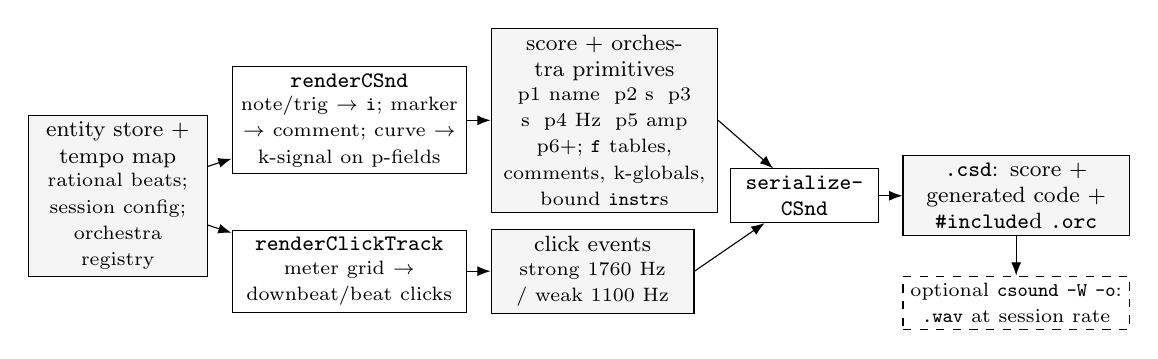
\begin{tikzpicture}[
  font=\footnotesize,
  box/.style={draw, align=center, inner sep=2.5pt, fill=white},
  data/.style={box, fill=gray!8},
  arrow/.style={-Latex}
]
\node[box, text width=28mm] (rend)
  {\texttt{renderCSnd}\\[-1pt]
   {\scriptsize note/trig $\to$ \texttt{i}; marker $\to$ comment;
    curve $\to$ k-signal on p-fields}};
\node[box, text width=28mm, below=7mm of rend] (click)
  {\texttt{renderClickTrack}\\[-1pt]
   {\scriptsize meter grid $\to$ downbeat/beat clicks}};
\node[data, text width=21mm, left=3mm of $(rend.west)!0.5!(click.west)$] (store)
  {entity store $+$ tempo map\\[-1pt]
   {\scriptsize rational beats; session config; orchestra registry}};
\node[data, text width=27mm, right=3mm of rend] (prim)
  {score $+$ orchestra primitives\\[-1pt]
   {\scriptsize p1 name\; p2 s\; p3 s\; p4 Hz\; p5 amp\; p6+;
    \texttt{f} tables, comments, k-globals, bound \texttt{instr}s}};
\node[data, text width=24mm, right=3mm of click] (cprim)
  {click events\\[-1pt]
   {\scriptsize strong 1760 Hz / weak 1100 Hz}};
\node[box, text width=17mm, right=3mm of $(prim.east)!0.5!(cprim.east)$] (ser)
  {\texttt{serialize-\\CSnd}};
\node[data, text width=27mm, right=3mm of ser] (csd)
  {\texttt{.csd}: score $+$ generated code $+$ \texttt{\#include}d
   \texttt{.orc}};
\node[box, dashed, text width=27mm, below=5mm of csd] (wav)
  {{\scriptsize optional \texttt{csound -W -o}: \texttt{.wav} at session rate}};
\draw[arrow] (store) -- (rend);
\draw[arrow] (store) -- (click);
\draw[arrow] (rend) -- (prim);
\draw[arrow] (click) -- (cprim);
\draw[arrow] (prim.east) -- (ser);
\draw[arrow] (cprim.east) -- (ser);
\draw[arrow] (ser) -- (csd);
\draw[arrow] (csd) -- (wav);
\end{tikzpicture}
\caption{Both Csound-family renderers share one serializer; source
instruments stay in external \texttt{.orc} files, and curve bindings add
generated copies without touching them.}
\label{fig:pipeline}
\end{figure}

Two decisions matter most. First, \emph{late conversion}: because onsets
stay Rational until this point, \texttt{p2}/\texttt{p3} are computed from
the compiled tempo map, \texttt{p4} from spelling and cents under the
session's \texttt{tuningA4}, and \texttt{p5} from the dynamic marking, all
at render time. Retuning a session to 432~Hz or editing its tempo specification
regenerates every second and every frequency without touching one entity.
Second, \emph{named instruments}: an orchestra registry is loaded from a
directory of \texttt{.orc} files, the filename being the stable id used
both in \texttt{instr} definitions and in entity payloads. No numeric
renumbering ever occurs, so the note

{\small\begin{verbatim}
i "sine_osc" 0. 4. 440. 0.65 0.5
\end{verbatim}}

\noindent
(A4, \emph{mf}, two whole notes at 120~BPM, actual paclet output) remains
readable and stable as the orchestra grows.

Curves reach the sounding notes through declared bindings: by default an
\texttt{amplitude} curve multiplies \texttt{p5}. For each affected instrument
the renderer copies the whole \texttt{instr} body from its source \texttt{.orc}
into a \emph{bound copy}, rewriting only the use-sites of the bound
p-fields---the control-signal globals multiply or replace them, everything else
(\texttt{pcount()} guards, envelopes, \texttt{limit()} clamps, the oscillator)
reproduced verbatim. Affected notes are re-pointed to this copy, and several
curves may compose on one p-field (in Fig.~\ref{fig:timeline}, two amplitude
curves and an \texttt{ampScale} curve into \texttt{p5}; \texttt{panSweep} and
\texttt{panDepth} into \texttt{p6}). Regenerated every render and never edited
at the source, the copy cannot drift. The serializer writes the globals and
generated instruments beside the registry's \texttt{\#include} lines, sorts
score statements by onset, and can compile the \texttt{.csd} to audio.

The same amplitude curve lives differently outside Csound. Projected to OSC it
is not bound into an instrument but sampled at the session control rate into
timed messages. A linear ramp over two seconds at $10$~Hz becomes a JSON event
list (fields \texttt{version}, \texttt{sampleRate}, \texttt{duration\_ms}, and
per-sample \texttt{events}), each event an OSC message---\texttt{time\_ms}~1900,
\texttt{address} \texttt{/param/amplitude}, \texttt{args}~\texttt{[0.95]}
(actual paclet output, excerpted\footnote{Full example artifacts (aggregated
\texttt{.csd}/\texttt{.wav}, click track, OSC JSON, notebook, \texttt{.orc}
instruments) and the four-backend synchrony demonstration are in the
supplementary folder: \url{\supplementaryurl}.}). The beat-space curve and tempo
map are the same as in the Csound projection; one binds the curve to a score
p-field, the other streams it as OSC messages in milliseconds---a genuinely
non-Csound artifact, the heterogeneity the architecture exists to make cheap.

\section{A Click Track from the Same Timeline}\label{sec:click}

Click tracks for mixed music are commonly rebuilt by hand in a DAW whenever the
score changes---precisely the divergence this architecture removes. The click
backend treats rehearsal audio as one more projection: it reads only the
authored meter entities and the tempo map, builds the measure grid, and emits
one short \texttt{i}~event per beat, accenting each downbeat. Every parameter is
session configuration---beat unit ($1/4$), click duration ($1/16$), strong/weak
frequencies ($1760/1100$~Hz), amplitudes ($0.9/0.45$), and pan---and the click
instrument itself is an ordinary three-line \texttt{.orc} file. Because the
renderer walks the same meter grid and tempo map as every other backend, meter
and tempo changes are followed with no additional authoring; for two $4/4$ bars
at 120~BPM it emits strong \texttt{i "click"} downbeats (0 and 2~s) and weak
intervening beats (full \texttt{.csd} and \texttt{.wav} in the supplementary
folder). In roughly 140 lines that reuse \texttt{serializeCSnd} unchanged
(Fig.~\ref{fig:pipeline}) and touch no line of Layers~I--II, the backend
inherits \texttt{\#include} handling and optional \texttt{.wav}
compilation---showing how cheaply a further projection follows once the
temporal core is shared. The genuinely different
time encodings, notation's divisions and OSC's milliseconds, belong to the
MusicXML and OSC contracts.

\section{Keeping the Projections Synchronous}

Because every backend reads the same rational onsets and the same compiled
tempo map, the projections cannot drift apart. Take one authored timeline---two
$4/4$ bars then $3/4$, $120$ then $90$~BPM---projected to all four backends. The
downbeat of bar~3 is Csound \texttt{p2}$=4.0$\,s, OSC \texttt{time\_ms}$=4000$,
and a strong click at $4.0$\,s, while MusicXML places it at bar~3, beat~1.
Editing the second tempo segment to $60$~BPM moves every later onset by the same
amount in all three time-domain backends (the note at beat $9/4$: $4.667 \to
5.0$\,s) while the MusicXML export is byte-identical: notation lives in beat
space, and seconds are bound only at render time. This four-backend synchrony
demonstration, before and after the edit, is in the supplementary material.

\section{Conclusions}

Temporal System contributes an architecture, not a synthesis method: an
immutable rational-beat store from which Csound scores, click tracks, notation,
and real-time event streams are compiled as unequal but coordinated projections,
Csound being the reference renderer that makes the contract concrete. There is
deliberately no MIDI backend---MusicXML covers notation, Csound fixed-media
synthesis, and OSC real-time control beyond MIDI's resolution. The paclet is
not yet released; its example artifacts are on Zenodo. Current
work stabilizes the MusicXML backend beyond beta and adds a hierarchical
generation layer above the store. Sixty years after \emph{Project~1} and the
Bell Labs note-lists, separating computed time from rendered sound still
pays---it lets one timeline become many renderings.

\begin{thebibliography}{99}

\bibitem{koenig} Koenig, G.M.: Project Two: A Programme for Musical
Composition. Electronic Music Reports 3, 4--161. Institute of Sonology,
Utrecht (1970)

\bibitem{tenney} Tenney, J.: Computer Music Experiences, 1961--1964.
Electronic Music Reports 1(1), 23--60. Institute of Sonology, Utrecht (1969)

\bibitem{mathews} Mathews, M.V.: The Technology of Computer Music. MIT
Press, Cambridge (1969)

\bibitem{csoundbook} Lazzarini, V., Yi, S., ffitch, J., Heintz, J.,
Brandtsegg, {\O}., McCurdy, I.: Csound: A Sound and Music Computing System.
Springer (2016)

\bibitem{openmusic} Assayag, G., Rueda, C., Laurson, M., Agon, C., Delerue,
O.: Computer-Assisted Composition at IRCAM: From PatchWork to OpenMusic.
Computer Music Journal 23(3), 59--72 (1999)

\bibitem{taube} Taube, H.: Notes from the Metalevel: Introduction to
Algorithmic Music Composition. Taylor \& Francis, London (2004)

\bibitem{music21} Cuthbert, M.S., Ariza, C.: music21: A Toolkit for
Computer-Aided Musicology and Symbolic Music Data. In: Proceedings of the
11th International Society for Music Information Retrieval Conference (ISMIR),
pp. 637--642. Utrecht (2010)

\bibitem{abjad} Ba{\v c}a, T., Oberholtzer, J.W., Trevi{\~n}o, J.,
Ad{\'a}n, V.: Abjad: An Open-Source Software System for Formalized Score
Control. In: Proceedings of the First International Conference on
Technologies for Music Notation and Representation (TENOR), pp. 162--169.
Paris (2015)

\bibitem{mei} Hankinson, A., Roland, P., Fujinaga, I.: The Music Encoding
Initiative as a Document-Encoding Framework. In: Proceedings of the 12th
International Society for Music Information Retrieval Conference (ISMIR),
pp. 293--298. Miami (2011)

\bibitem{verovio} Pugin, L., Zitellini, R., Roland, P.: Verovio: A Library
for Engraving MEI Music Notation into SVG. In: Proceedings of the 15th
International Society for Music Information Retrieval Conference (ISMIR),
pp. 107--112. Taipei (2014)

\bibitem{bach} Agostini, A., Ghisi, D.: A Max Library for Musical Notation
and Computer-Aided Composition. Computer Music Journal 39(2), 11--27 (2015)

\bibitem{tidal} McLean, A.: Making Programming Languages to Dance to: Live
Coding with Tidal. In: Proceedings of the 2nd ACM SIGPLAN International
Workshop on Functional Art, Music, Modeling \& Design (FARM~'14), pp. 63--70.
ACM, New York (2014)

\bibitem{good} Good, M.: MusicXML for Notation and Analysis. In: Hewlett,
W.B., Selfridge-Field, E. (eds.) The Virtual Score: Representation,
Retrieval, Restoration, pp. 113--124. MIT Press, Cambridge (2001)

\bibitem{osc} Wright, M., Freed, A.: Open SoundControl: A New Protocol for
Communicating with Sound Synthesizers. In: Proceedings of the International
Computer Music Conference, pp. 101--104. Thessaloniki (1997)

\bibitem{wolfram} Wolfram Research: Wolfram Language and Paclet
Documentation. \url{https://reference.wolfram.com/language/}

\end{thebibliography}

\end{document}
